\documentclass[conference]{IEEEtran}

\usepackage{amsmath,amssymb}
\usepackage{booktabs}
\usepackage{graphicx}
\usepackage{microtype}
\usepackage{xcolor}
\usepackage{url}

\graphicspath{{figures/}}
\newcommand{\wq}{w_q}
\newcommand{\sigw}{\sigma_{w_q}}

\title{Learning When Black-Hole Hair Is Observable\\
from Synthetic Ringdown Waves}

\author{
\IEEEauthorblockN{Ariadna Uxue Palomino Ylla}
\IEEEauthorblockA{Nagoya University\\
Nagoya, Japan\\
ariadnaepy@gmail.com}
}

\begin{document}
\maketitle

\begin{abstract}
We ask when a synthetic black-hole ringdown contains enough information to
recover the Kiselev parameters $(k,\wq)$, and when the inverse map is too
ill-conditioned for finite-precision inference. To prevent repeated mode
realizations of one spacetime from leaking across data partitions, we use
grouped physical cross-validation and fit waveform PCA only on training folds.
A waveform-only random forest reaches $R^2(k)=0.8960$ and
$R^2(\wq)=0.9587$; the original synthetic-geodesic proxy experiment raises these scores to
$0.9793$ and $0.9891$ with histogram gradient boosting. More importantly, an
all-feature random-forest classifier reproduces a Fisher/Jacobian
observability boundary with macro F1 $=0.9928$, using
$\sigw>0.3$ at one-percent relative observable precision as the weak-
identifiability criterion. In a companion scalar/proxy identifiability
experiment, adding synthetic geodesic features reduces mean absolute $\wq$
error from $0.0225$ to $0.0143$ and improves local conditioning near $k=0$.
We subsequently replace those proxies with validated timelike-emitter and
three-dimensional null-geodesic shooting. On a 121-point physical Kiselev
grid, adding photon geometry to ringdown improves the median minimum singular
value by $4.54\times$ and median conditioning by $2.28\times$ relative to
ringdown alone. This is a controlled physical-identifiability benchmark, not
an observational constraint; final inverse-ML generalization on the physical
feature table remains a separate validation stage.
\end{abstract}

\begin{IEEEkeywords}
scientific machine learning, inverse problems, black-hole ringdown,
identifiability, grouped validation, Fisher information
\end{IEEEkeywords}

\section{Introduction}
This paper studies a specific inverse problem: recovering the Kiselev
parameters $(k,\wq)$ from the frequency and damping morphology of synthetic
ringdown curves. In the eikonal limit, quasinormal frequencies are related to
the orbital frequency and instability exponent of an unstable circular null
geodesic \cite{cardoso2009geodesic,palominoylla2026ringdown}. The relation gives a transparent
simulator in which machine-learning behavior can be compared directly with the
local derivatives of the observable map.

In this setting, a high $R^2$ can mean either genuine recovery of Kiselev
parameters or interpolation across repeated mode realizations of the same
spacetime. Each $(k,\wq)$ point produces several curves through different
angular indices $\ell$ and overtones $n$; a row-wise split can therefore place
nearly identical physical systems in training and test sets. Even after that
leakage is removed, a model may interpolate accurately in most of the grid
while becoming unreliable where the inverse map is locally ill-conditioned.
Our central question is consequently: when does a synthetic ringdown contain
enough information to infer Kiselev hair parameters, and when are
finite-precision errors amplified too strongly?

We address these issues in a synthetic Kiselev black-hole study. The Kiselev
solution is a static, spherically symmetric geometry containing an amplitude
$k$ and state parameter $\wq$ \cite{kiselev2003quintessence}. Our simulator uses
leading-order analytic shifts rather than a dedicated perturbative solver. We
generate damped curves, enforce grouped physical validation, fit PCA within
training folds, and compare several inverse models. We then change the target:
instead of predicting only $(k,\wq)$, a classifier predicts whether $\wq$ is
practically identifiable under a stated precision model. A numerical
Fisher/Jacobian calculation provides the scientific label and an analytic
interpretation of failures.

We address that question through the original inverse-learning study and a
subsequent physical-validation program:
\begin{itemize}
  \item grouped physical validation for waveform-to-hair inference, with PCA
  fitted inside each training fold;
  \item regression from synthetic leading-eikonal curves to $(k,\wq)$;
  \item Fisher/Jacobian labels for weakly identifiable regions;
  \item comparison of waveform-only, scalar, and synthetic geodesic-proxy
  representations; and
  \item joint interpretation of ML errors and local singular-value diagnostics;
  \item Hamiltonian timelike and null shooting with physical phase beginning
  at apocentre, $\phi=\pi$;
  \item Schwarzschild, small-$k$, and fixed-$k$ $\wq$-sensitivity validation;
  and
  \item two-dimensional physical Jacobian and observable-complementarity maps.
\end{itemize}

The central result is not the regression score by itself. The more useful
outcome is that a learned classifier reproduces the Fisher/Jacobian
observability boundary, separating regions where the waveform-to-hair map is
informative from regions where finite-precision errors are amplified.

\section{Synthetic Leading-Eikonal Waveform Dataset}
\subsection{Static Kiselev simulator}
We set the mass scale to $M=1$ and sample a dense grid
\begin{equation}
 k\in[-0.04,0.04], \qquad \wq\in[-1.4,1.4].
\end{equation}
The underlying Kiselev metric family motivates the dependence on both
parameters \cite{kiselev2003quintessence}; the present implementation uses
analytic leading-order expressions for the photon-orbit radius shift
$\Delta r$, orbital frequency $\Omega$, and Lyapunov exponent $\lambda$.
Non-finite or non-positive leading-order points are excluded.
The broad $\wq$ interval is used as a controlled benchmark of inverse-map
geometry and is not intended to identify every sampled point with the standard
quintessence regime.

For each retained physical point, the eikonal mapping is
\begin{equation}
 \omega_R=\ell\Omega,\qquad
 \gamma=(n+\tfrac{1}{2})\lambda ,
\end{equation}
and the synthetic time-domain curve is
\begin{equation}
 \Psi(t)=\exp(-\gamma t)\cos(\omega_R t).
 \label{eq:ringdown}
\end{equation}
We use $\ell\in\{4,5,10,20\}$, $n\in\{0,1\}$, and 512 uniformly spaced time
samples. The eight mode curves are averaged into one 512-sample multi-mode
morphology per physical point for the waveform-to-hair experiment. This
aggregation prevents repeated modes from being treated as independent target
samples while retaining their combined morphology. The equal-weight average is
a benchmark feature construction rather than an astrophysical multimode
waveform with physically inferred amplitudes and phases.

\subsection{Feature families}
Five representations are evaluated: (A) the raw waveform; (B) waveform PCA;
(C) waveform PCA with $(\Omega,\lambda)$; (D) waveform PCA with four synthetic
geodesic proxies; and (E) waveform PCA with all current scalars and proxies.
The current scalars are $\Omega$, $\lambda$, $\omega_R$, $\gamma$, and
$\Delta r$.

The additional features are smooth proxies for impact parameter, screen
coordinate, propagation-time delay, and a redshift curve. They exercise a
replaceable multi-observable interface and test whether parameter dependence
not reducible to $(\Omega,\lambda)$ can improve conditioning. They should not be
interpreted as geodesic-shooting or ray-tracing predictions.

The later physical-shooting features are a distinct family, not a relabeling
of these proxies. They are derived from integrated emitter and photon
trajectories and include redshift, impact parameter, signed observer-tetrad sky
coordinates, propagation delay, and arrival-time curves. The regression values
below remain the historical proxy benchmark.

\section{Leakage-Aware Inverse-Learning Protocol}
\subsection{Grouped physical validation}
The grouping variable is the physical pair $(k,\wq)$; neither $\ell$ nor $n$
defines a new physical system. Grouped cross-validation therefore assigns all
mode realizations of one physical point to exactly one fold. This is the central
leakage control. For the zero-noise headline experiment, PCA is fitted on clean
training curves. In the noise study, independent noise is added to training
and test curves, and PCA is fitted only on the noisy training fold at each
noise level. PCA never sees held-out test data. This follows the general
train-transform-test discipline implemented with scikit-learn
\cite{pedregosa2011scikit}.

Regression candidates are Ridge, random forest, histogram gradient boosting,
and a multilayer perceptron. Classification candidates are logistic regression,
random forest, histogram gradient boosting, and a multilayer perceptron.
Random forests provide a robust nonlinear baseline \cite{breiman2001random};
gradient boosting supplies a complementary additive-tree model
\cite{friedman2001greedy}. Hyperparameters are deliberately modest because the
scientific question concerns information content rather than model scaling.

Regression is measured using $R^2$, mean absolute error (MAE), and root mean
squared error for each target. Classification is measured with accuracy, macro
F1, and a confusion matrix. Gaussian waveform noise at 0, 0.5, 1, 3, and 5
percent of the per-waveform standard deviation is injected before PCA or direct
waveform input.

\subsection{Practical-identifiability label}
Let the local observable vector be
\begin{equation}
 {\bf y}(k,\wq)=(\Omega,\lambda,\omega_R,\gamma,\Delta r)^{\mathsf T}.
\end{equation}
Finite differences give the Jacobian
\begin{equation}
 J=\frac{\partial{\bf y}}{\partial(k,\wq)} .
\end{equation}
Under independent one-percent relative errors, with a small absolute floor for
zero-valued shifts, we whiten the Jacobian as
\begin{equation}
 \widetilde J=C_y^{-1/2}J=U\,{\rm diag}(s_i)\,V^{\mathsf T}.
\label{eq:fisher}
\end{equation}
Singular values below
$\max(\epsilon_{\rm abs},\epsilon_{\rm rel}s_{\max})$, with
$\epsilon_{\rm rel}=10^{-8}$ and $\epsilon_{\rm abs}=0$, define the numerical
null space. This tolerance is supported by derivative convergence: five-point
and three-point whitened Jacobians differ relatively by at most
$9.31\times10^{-9}$ at representative near-degenerate points, and scaling both
finite-difference steps from $0.25$ to $4$ leaves all labels unchanged. If the
explicit $\wq$ direction overlaps the numerical null space, we set
$\sigw=\infty$ and mark the parameter structurally or numerically
non-identifiable. Otherwise the covariance is assembled from retained
singular directions,
$\Sigma_\theta=V_r{\rm diag}(s_r^{-2})V_r^{\mathsf T}$. This avoids the
incorrect finite zero uncertainty that a bare pseudoinverse assigns to a
discarded parameter direction.

At exactly $k=0$, the observables have no $\wq$ dependence, the Jacobian has
rank one, and $\sigw=\infty$. At small nonzero $|k|$, by contrast, the
Jacobian can remain full rank while producing a large but finite uncertainty.
We call this practical weak identifiability, labeling a point weak when
\begin{equation}
 \sigw=\sqrt{(\Sigma_\theta)_{\wq\wq}}>0.3 .
 \label{eq:weak}
\end{equation}
This criterion labels 57.6\% of proxy-valid physical points as weakly
identifiable. It is a simulator-specific, precision-dependent phase diagram,
not an observational posterior.

\subsection{Reproducibility and audit trail}
The experiment is implemented in the open research prototype
\texttt{black-hole-hair-ml} \cite{palomino2026bhhairml}. Configuration files
record the dense parameter ranges, mode indices, number of time samples, PCA
dimension, model settings, and noise levels. Each run exports fold-level
metrics, out-of-fold predictions, noise tables, paired PNG/PDF figures, and an
automatically generated scope-aware report. The physical group identifier is
stored explicitly with predictions, allowing a post-run check that no group
crosses the train/test boundary. The PCA object is constructed inside the fold
loop rather than fitted once on the full dataset. These implementation details
are important because a numerically strong result would not be scientifically
interpretable if preprocessing or repeated-mode leakage exposed test
information during training.

The present workshop draft reports the completed default experiment rather than
a hyperparameter optimization study. Model families were compared under the
same grouped partitions, and the best named estimators are selected from that
controlled comparison. The feature comparison reports the best mean grouped-CV
score for each feature-set/target pair.

\section{Waveform-to-Hair Prediction Results}
Table~\ref{tab:main} summarizes the main grouped results. Waveform morphology
alone is informative: the random forest reaches $R^2(k)=0.8960$ and
$R^2(\wq)=0.9587$. Because Eq.~\eqref{eq:ringdown} is fully determined by
$(\Omega,\lambda,\ell,n)$, this performance measures how well the model inverts
the frequency and damping morphology within the sampled simulator. It does not
demonstrate additional physical information in the curve.

\begin{table}[t]
\caption{Grouped waveform-to-hair results. Geodesic features are synthetic
proxies, not physical ray-tracing outputs.}
\label{tab:main}
\centering
\begin{tabular}{lcc}
\toprule
Input and best regressor & $R^2(k)$ & $R^2(\wq)$\\
\midrule
Waveform only, random forest & 0.8960 & 0.9587\\
Waveform + proxies, HistGB & 0.9793 & 0.9891\\
\bottomrule
\end{tabular}
\end{table}

\begin{figure}[t]
\centering
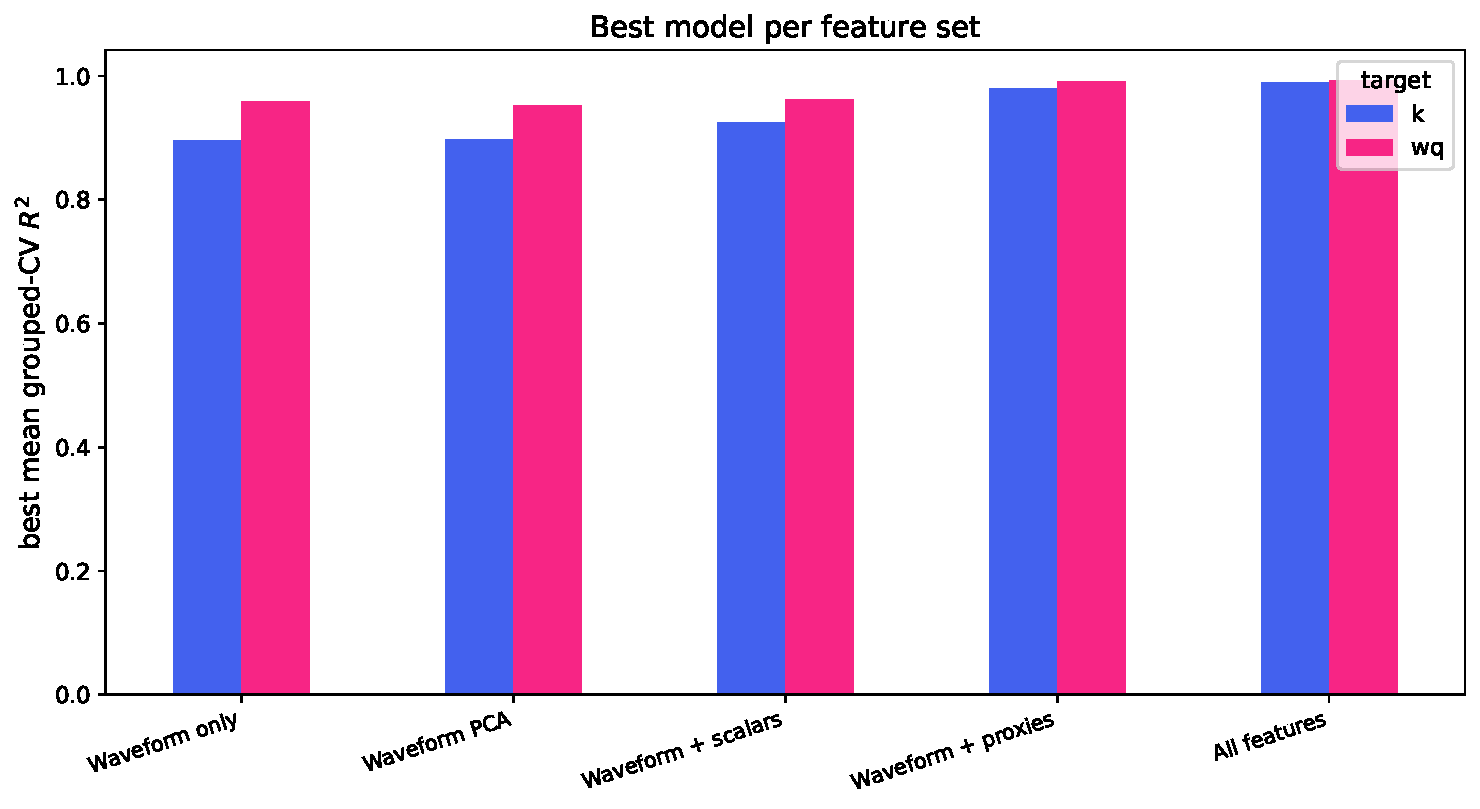
\includegraphics[width=\columnwidth]{waveform_to_hair_feature_comparison.pdf}
\caption{Grouped-CV feature comparison using the best model for each
feature-set/target pair. ``Proxies'' denotes synthetic geodesic features rather
than physical shooting or ray tracing.}
\label{fig:features}
\end{figure}

Adding proxy observables raises the jointly selected model scores to $0.9793$
and $0.9891$ with histogram gradient boosting. Figure~\ref{fig:features} gives
the complementary best-per-target comparison across representations. Within
this simulator, additional parameter dependence improves inverse recovery. The
physical analysis below tests whether validated observables retain that
advantage; final inverse-model generalization is not inferred from the Jacobian
alone.

The optional true-versus-predicted diagnostic in
Fig.~\ref{fig:truepred} shows the held-out structure for the best all-feature
model. Residuals are not uniform over parameter space; this motivates the
observability-classification task rather than treating a global score as a
complete scientific result.

\begin{figure}[t]
\centering
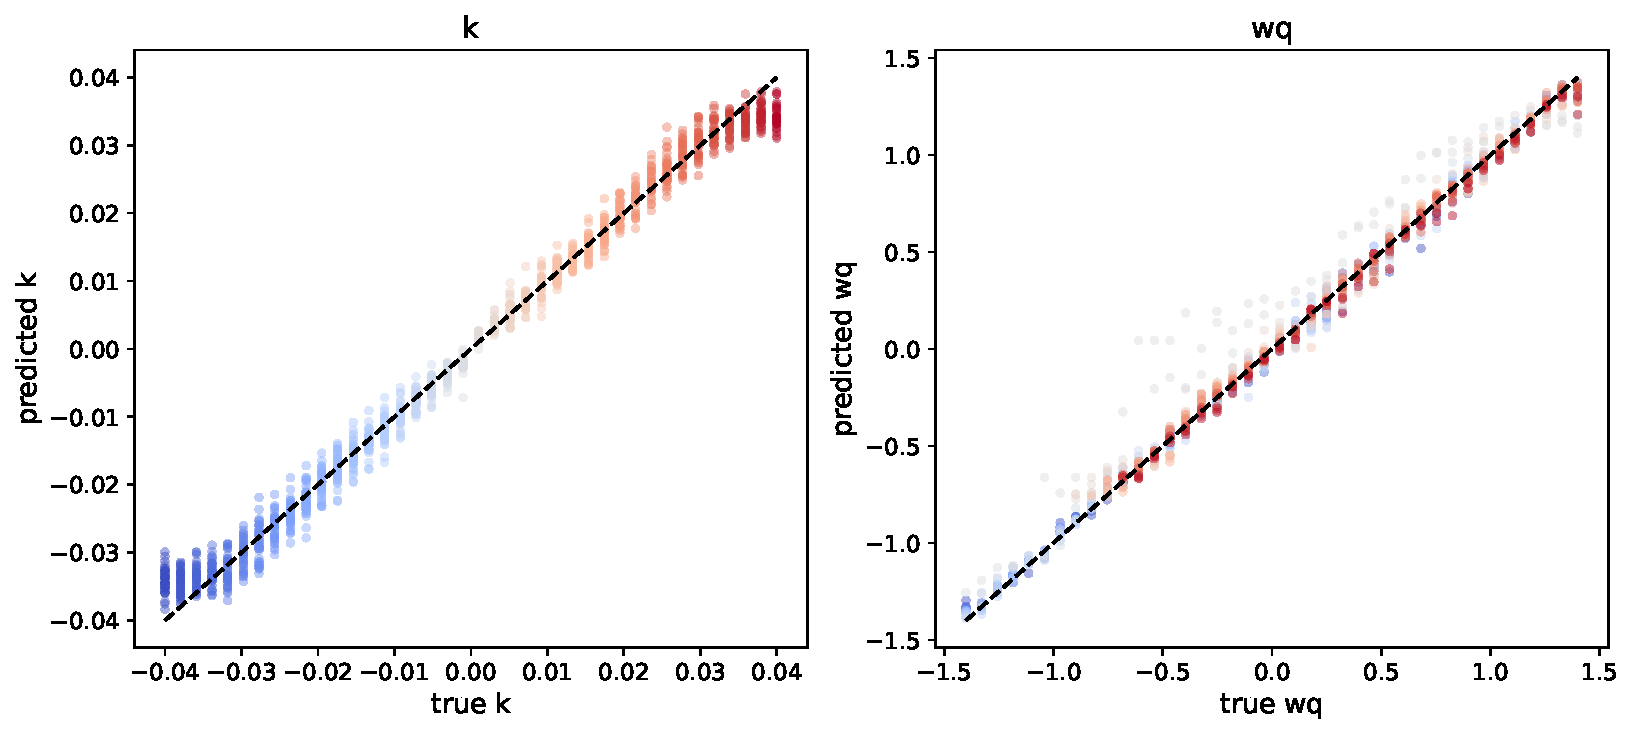
\includegraphics[width=\columnwidth]{waveform_to_hair_true_vs_pred.pdf}
\caption{True versus grouped-CV predicted $k$ and $\wq$ for the all-feature
histogram-gradient-boosting model, including waveform PCA, scalars, and
synthetic geodesic proxies.}
\label{fig:truepred}
\end{figure}

Waveform-only $\wq$ MAE rises by more than 25\% at the first tested nonzero
noise level, 0.5\%. This sensitivity should not be interpreted as a detector
threshold: the perturbation is idealized Gaussian noise on normalized
simulator curves and omits calibration, colored noise, mode uncertainty,
start-time selection, and waveform systematics.

\section{Learning Observability and Analytic Identifiability}
\begin{figure*}[t]
\centering
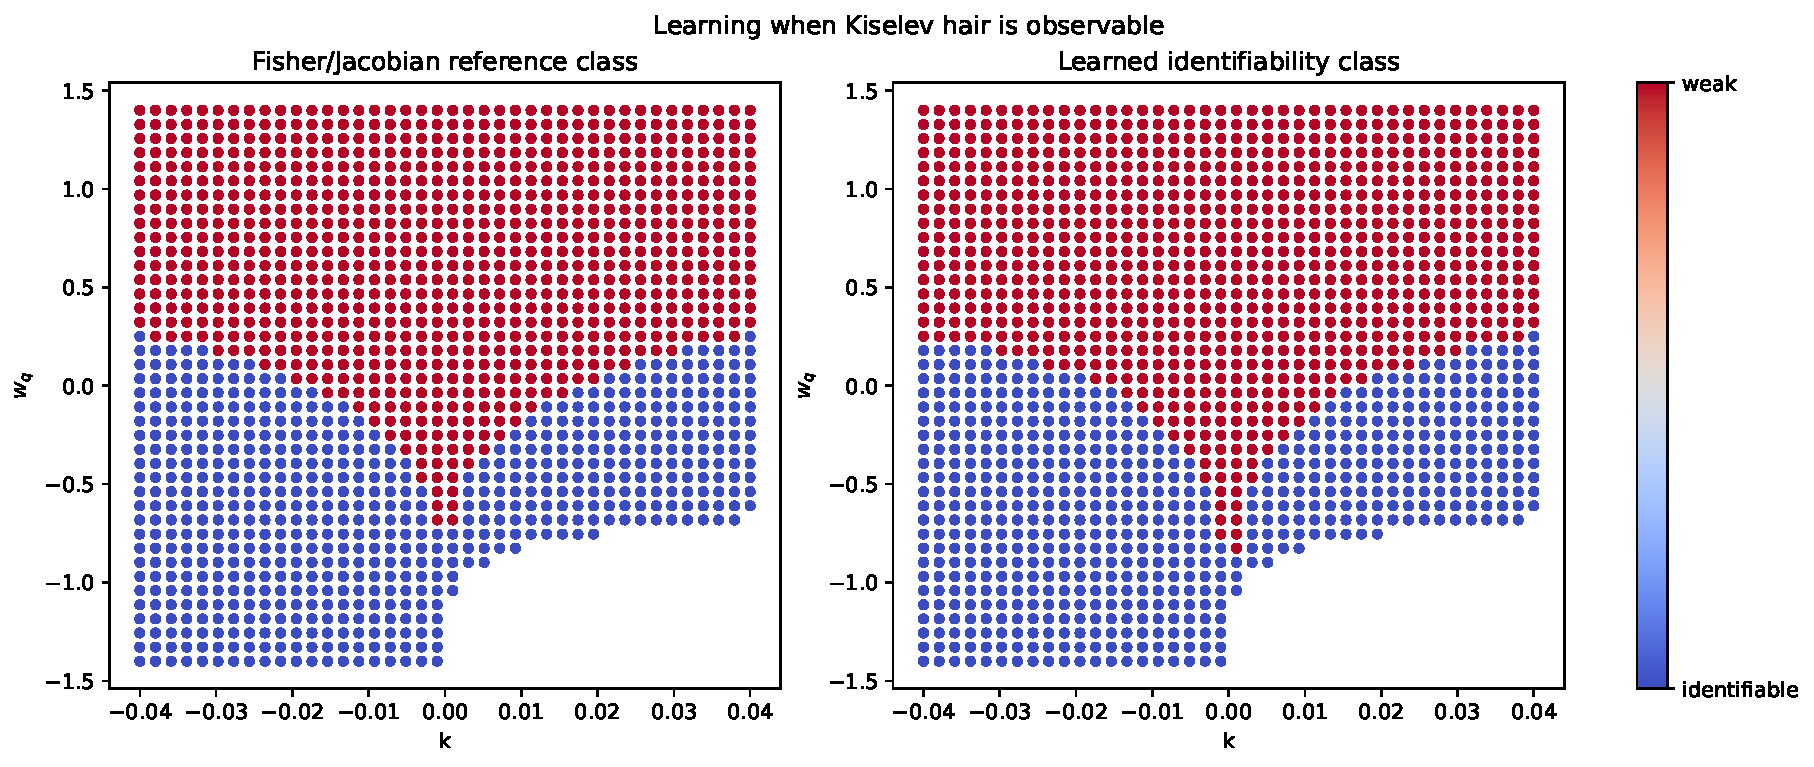
\includegraphics[width=0.88\textwidth]{learning_when_hair_is_observable_rank_aware.pdf}
\caption{True Fisher/Jacobian identifiability class (left) and grouped-CV
prediction (right). Weak identifiability means $\sigw>0.3$ under 1\% relative
observable precision. The all-feature random-forest classifier reaches macro
F1 $=0.9928$. The independently verified $k=0$ limit is Schwarzschild; the
nontrivial result shown here is the learned finite-precision boundary at small
nonzero $|k|$.}
\label{fig:observable}
\end{figure*}

Figure~\ref{fig:observable} compares the analytic class with predictions from
the best all-feature random-forest classifier. Its macro F1 is 0.9928. The
model captures both the broad transition in $\wq$ and the narrow structure
around small $|k|$. This is the central result: the classifier recovers where
the inverse problem is informative and where finite-precision uncertainty is
strongly amplified, rather than merely returning a parameter estimate.

An independently evaluated $k=0$ limit provides a structural sanity check: the
metric reduces to Schwarzschild and $\wq$ becomes unobservable. The nontrivial
result shown by the sampled grid is the finite-width weak-identifiability
region at small nonzero $|k|$.

\begin{figure*}[t]
\centering
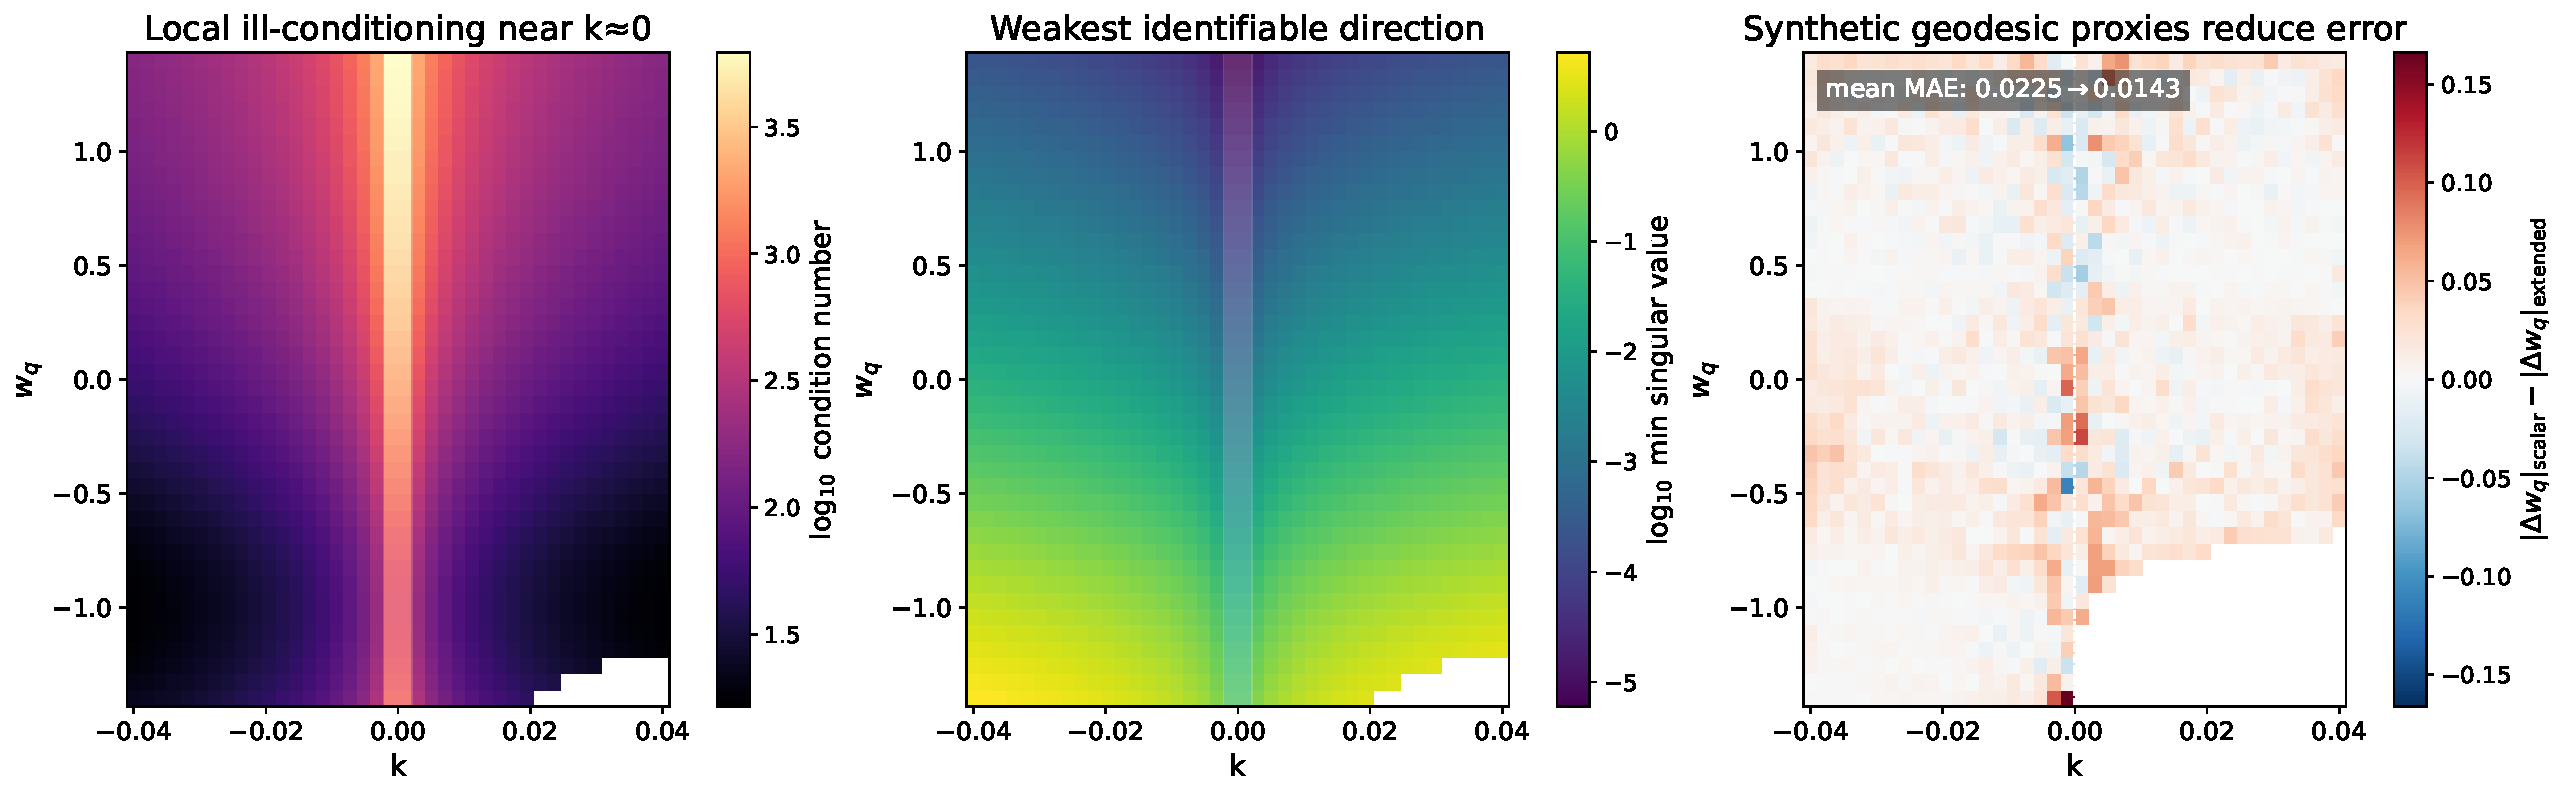
\includegraphics[width=0.98\textwidth]{kiselev_identifiability_lens.pdf}
\caption{Analytic identifiability lens. Left: Jacobian condition number.
Center: minimum singular value. Right: reduction in $\wq$ error after adding
synthetic geodesic proxies. The proxies are not physical ray-tracing or
shooting outputs.}
\label{fig:lens}
\end{figure*}

A companion proxy-identifiability experiment provides a complementary view of
this boundary in Fig.~\ref{fig:lens}. Large condition number marks amplification
of observable perturbations in the inverse problem, while the minimum singular
value measures the weakest local parameter direction. In that companion
scalar/proxy experiment, proxy augmentation reduces mean absolute $\wq$ error
from 0.0225 to 0.0143. In a near-$k=0$ band, the median minimum singular value
increases by approximately $12\times$, and the median condition number
improves by approximately $2.13\times$. Improvement at small nonzero $k$ does
not remove the independently verified exact-$k=0$ rank loss.

The agreement between learned classification and analytic sensitivity is more
scientifically informative than the regression score alone. It distinguishes
model failure from an inverse map whose local geometry suppresses information.
At the same time, the comparison remains internal to the assumed formulas and
error model. A different observable covariance or a validated perturbative
spectrum would move the practical boundary.

\section{Validated Physical Geodesic Shooting}
The proxy experiment motivated a separate physical calculation in the static
Kiselev metric
\begin{equation}
 ds^2=-f(r)dt^2+\frac{dr^2}{f(r)}+r^2d\Omega_2^2,
 \quad f(r)=1-\frac{2M}{r}-\frac{k}{r^{1+3\wq}}.
\end{equation}
An equatorial timelike emitter is evolved with conserved energy and angular
momentum from apocentre. The saved coordinate azimuth begins at $\phi=\pi$,
with $r=r_a$, $p_r=0$, and emission time and proper time zero. Coordinate
$\phi$ is not a Newtonian anomaly, so radial turning points are detected from
$p_r=0$ rather than imposed at multiples of $2\pi$.

Photons use a three-dimensional Cartesian null Hamiltonian,
\begin{equation}
 H_\gamma=\frac12\left[-\frac{1}{f}+\mathbf p^2+
 (f-1)(\mathbf n\!\cdot\!\mathbf p)^2\right]=0,
\end{equation}
and a two-angle root solve targets the static-observer plane. The direct branch
exports redshift $1+z=\omega_{\rm emit}/\omega_{\rm obs}$, conserved impact
parameter, signed observer-tetrad sky coordinates, propagation and excess
delay, and direct arrival time. An independent curve uses
\begin{equation}
 T_z(\phi)=\int_{\tau(\pi)}^{\tau(\phi)}(1+z)\,d\tau_{\rm emit},
\end{equation}
with only the common additive constant removed. Failed phases are reported,
not interpolated or replaced by proxy values.

For the Schwarzschild benchmark ($M=1$, $r_p=8M$, $r_a=12M$, observer at
$(0,0,-80M)$), all 322 rays across two arbitrary $\wq$ labels succeed and all
observables agree exactly between labels. Maximum hit, timelike-constraint,
null-constraint, and impact-drift errors are respectively
$3.85\times10^{-8}$, $2.01\times10^{-13}$, $7.20\times10^{-12}$, and
$1.78\times10^{-11}$. The arrival integral converges at approximately second
order. Pericentre is at $\phi=8.28375$ and the radial azimuthal period is
$10.28431$, giving physical apsidal advance $4.00113$.

At fixed $\wq=-0.5$, changing $k$ from zero to $10^{-3}$ produces resolved
changes in every selected orbital, redshift, photon-geometry, and timing
observable; the apsidal advance changes by 0.12767. At fixed $k=10^{-3}$,
changing $\wq$ from $-0.5$ to $-2/3$ changes the maximum redshift by 0.07341,
impact parameter by 0.30504, excess delay by 3.2342, and relative arrival time
by 1.6523. These ratios establish numerical resolvability, not observational
signal significance.

\begin{figure}[t]
\centering
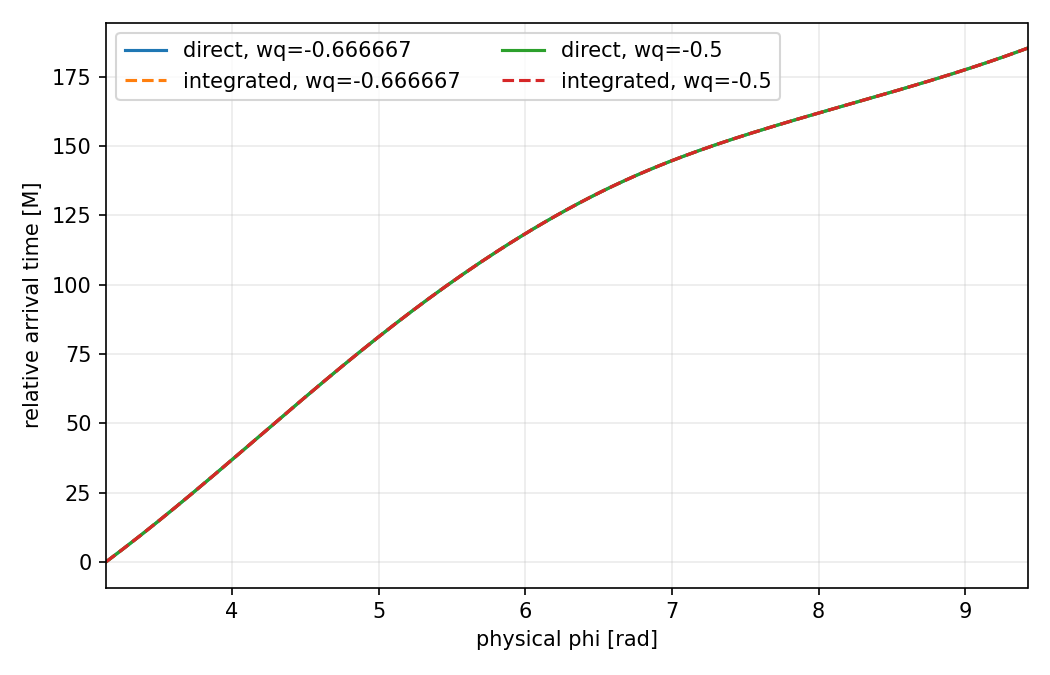
\includegraphics[width=\columnwidth]{physical_schwarzschild_arrival_validation.png}
\caption{Schwarzschild direct and integrated-redshift arrival curves. The
trapezoidal residual is reported rather than forced to zero.}
\label{fig:physical-schwarzschild}
\end{figure}

\begin{figure}[t]
\centering
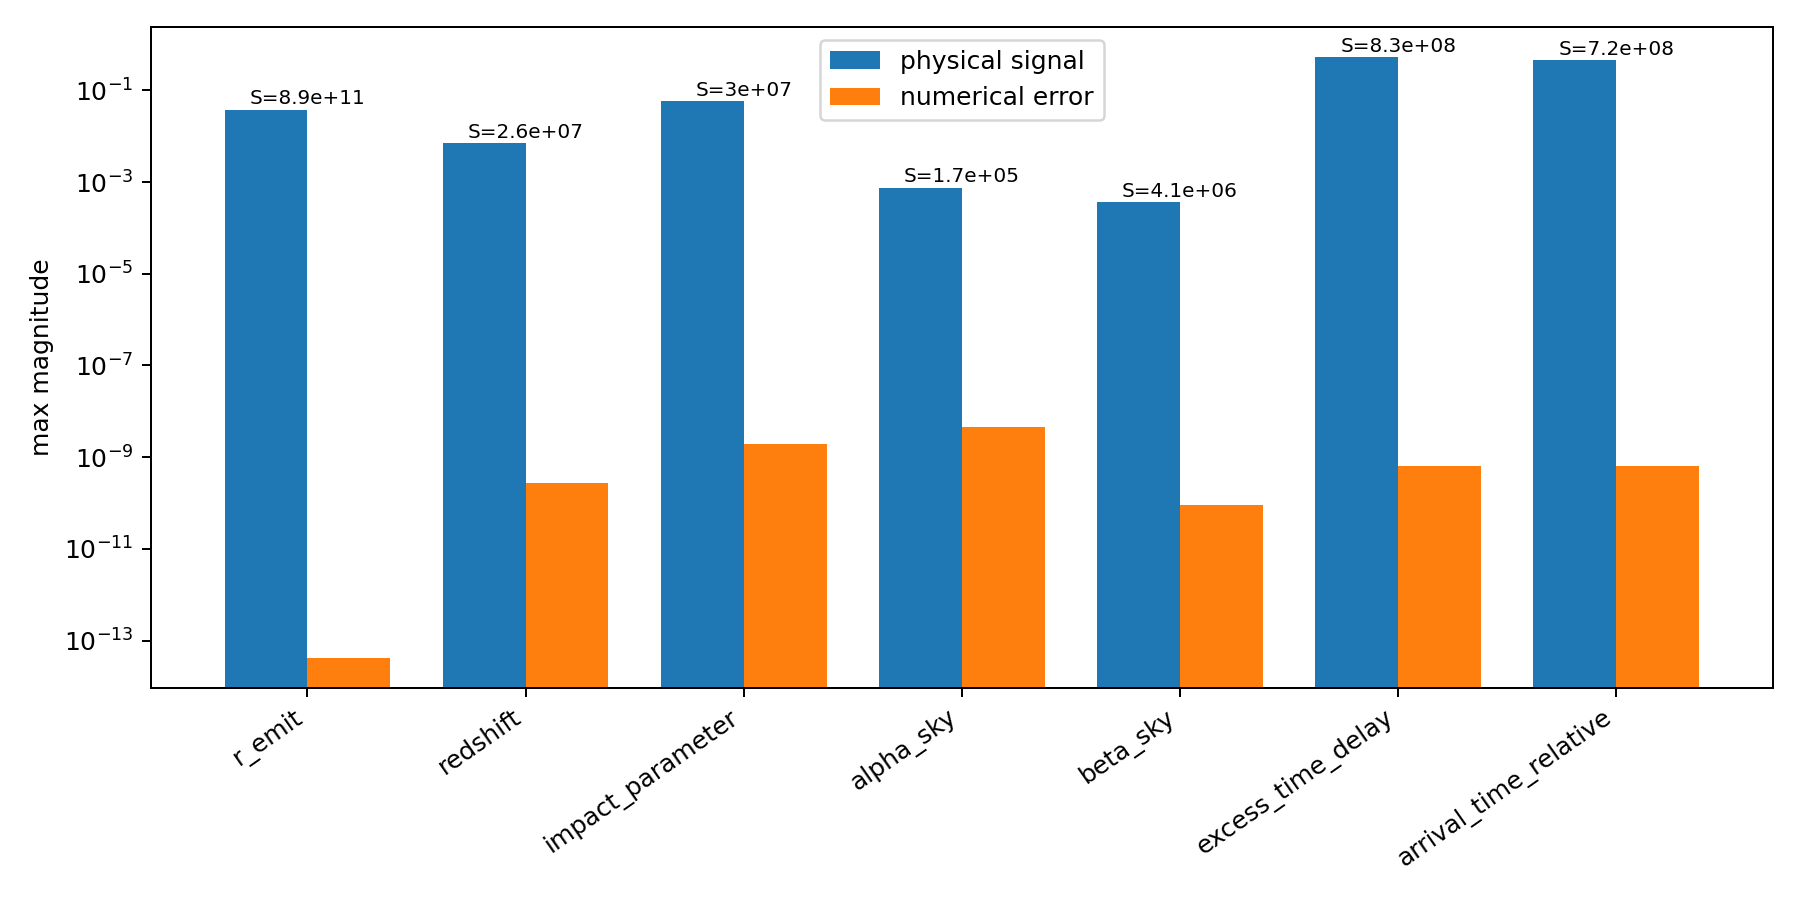
\includegraphics[width=\columnwidth]{physical_small_k_signal_validation.png}
\caption{First nonzero-$k$ physical differences relative to numerical error.}
\label{fig:physical-small-k}
\end{figure}

\begin{figure}[t]
\centering
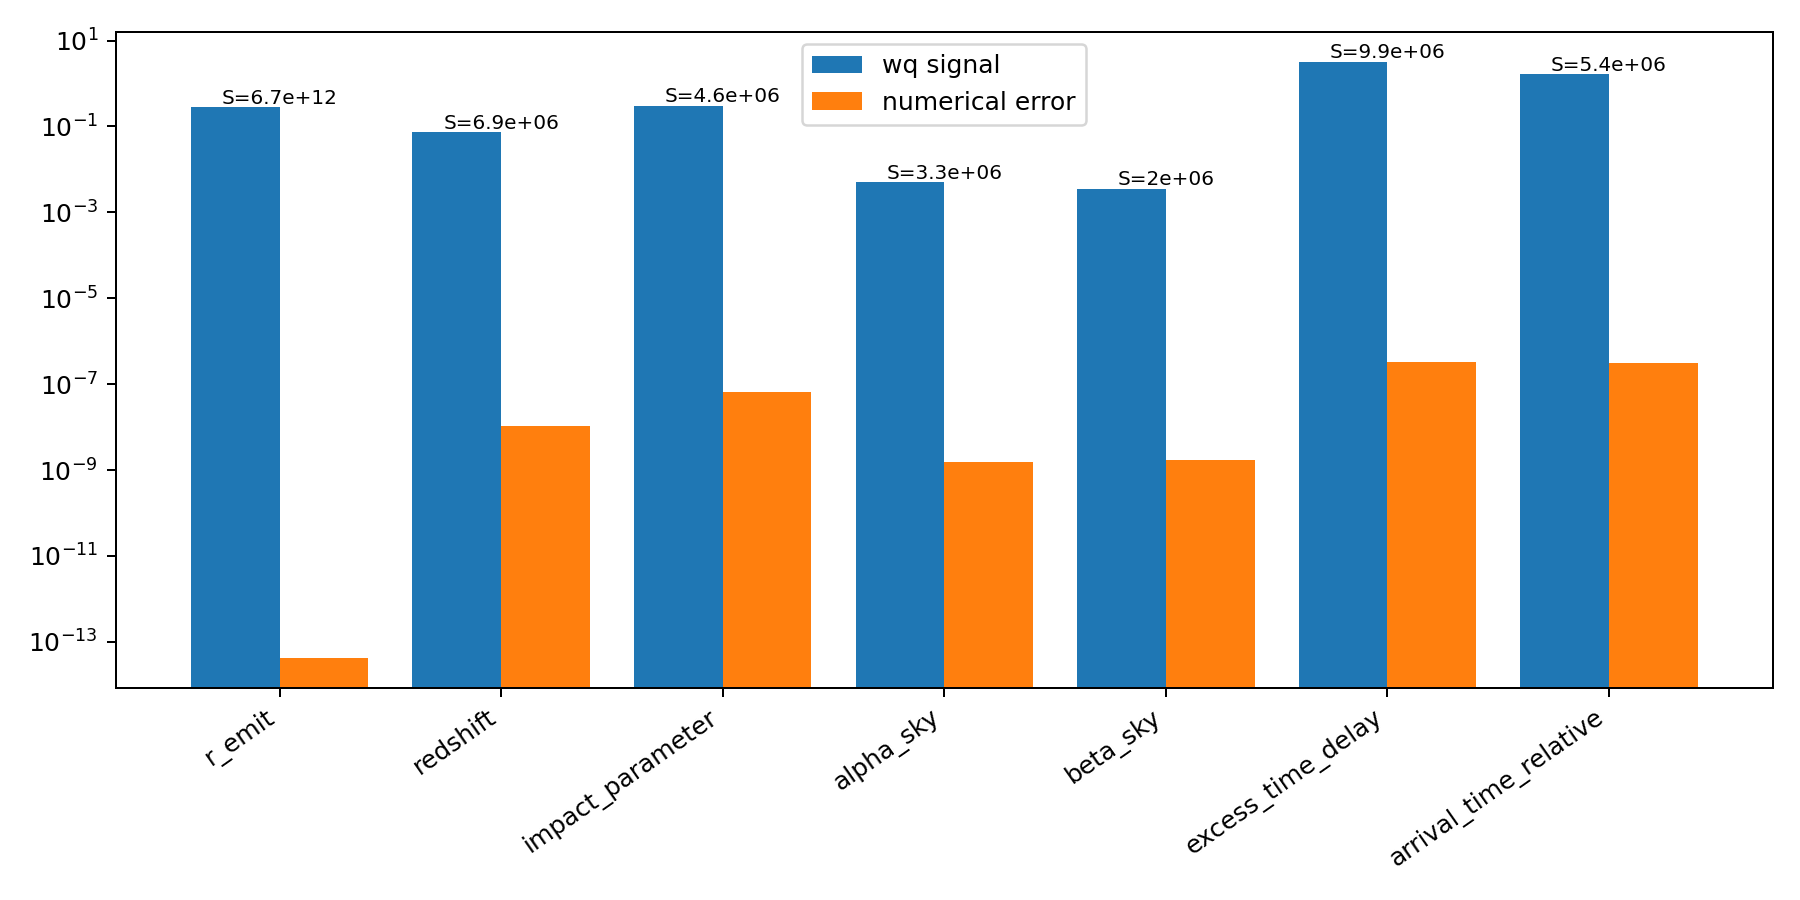
\includegraphics[width=\columnwidth]{physical_wq_sensitivity.png}
\caption{Fixed-$k$ physical sensitivity to changing $\wq$.}
\label{fig:physical-wq}
\end{figure}

\section{Physical Observable Complementarity Across Parameter Space}
Local standardized sensitivity vectors show that large responses may still be
nearly collinear. Timing has a large response but a sensitivity-vector angle
of $178.76^\circ$ and condition number 1275.5; photon geometry has the most
distinct tested direction ($159.37^\circ$, condition number 81.4). Adding more
signals can therefore add redundancy rather than independent information.

\begin{figure}[t]
\centering
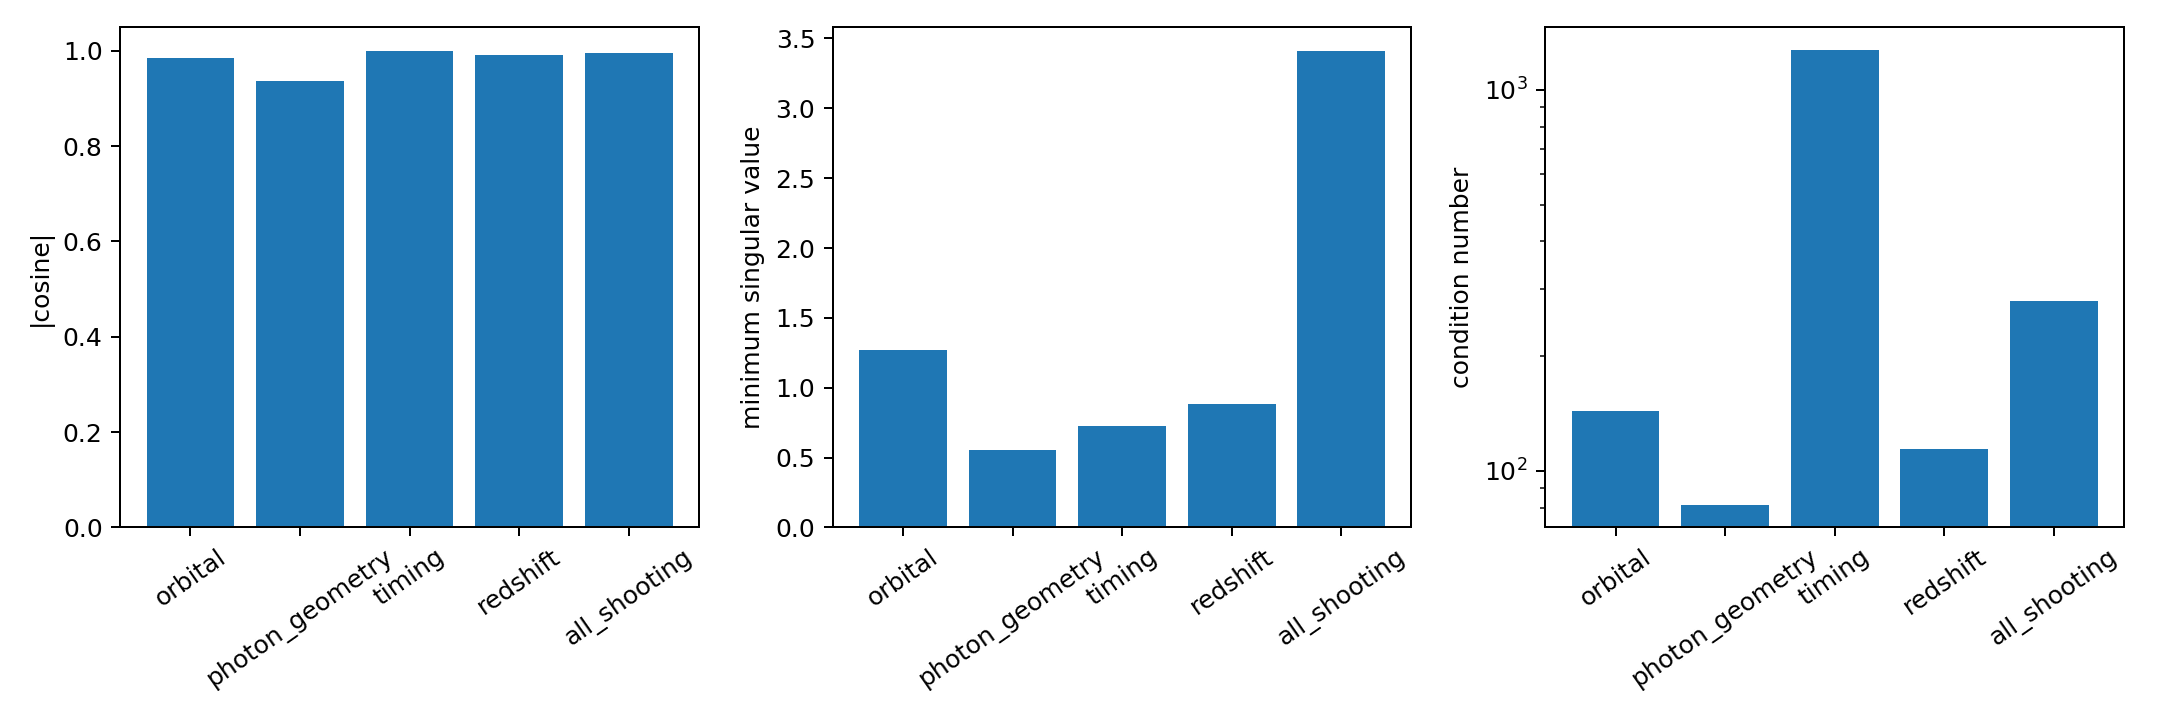
\includegraphics[width=\columnwidth]{physical_local_sensitivity_comparison.png}
\caption{Local sensitivity and conditioning by physical observable group.}
\label{fig:physical-local}
\end{figure}

A 9-by-9 admissibility scan identified 77 safe points, four invalid physical
points, and no software failures. The selected 11-by-11 science grid contains
121 accepted systems over $0\leq k\leq0.0025$ and
$-0.7125\leq\wq\leq-0.45$. At $k=0$, the metric is independent of $\wq$ and
\begin{equation}
 \frac{\partial\mathbf O}{\partial\wq}=0,
\end{equation}
so exact rank loss is required physically. Twenty-seven 161-phase checks change
the minimum singular value by at most 0.0401\% and the condition number by at
most 0.0713\%.

Across the grid, ringdown plus all shooting has median minimum singular value
1.5312 and median condition number 4.4974. Ringdown plus photon geometry gives
1.2326 and 4.0731, while all shooting gives 0.9723 and 6.0207. Relative to
ringdown alone, ringdown plus photon geometry improves median minimum singular
value by $4.54\times$ and median conditioning by $2.28\times$. Independent
parameter direction, rather than feature count or signal amplitude, controls
the gain.

\begin{figure*}[t]
\centering
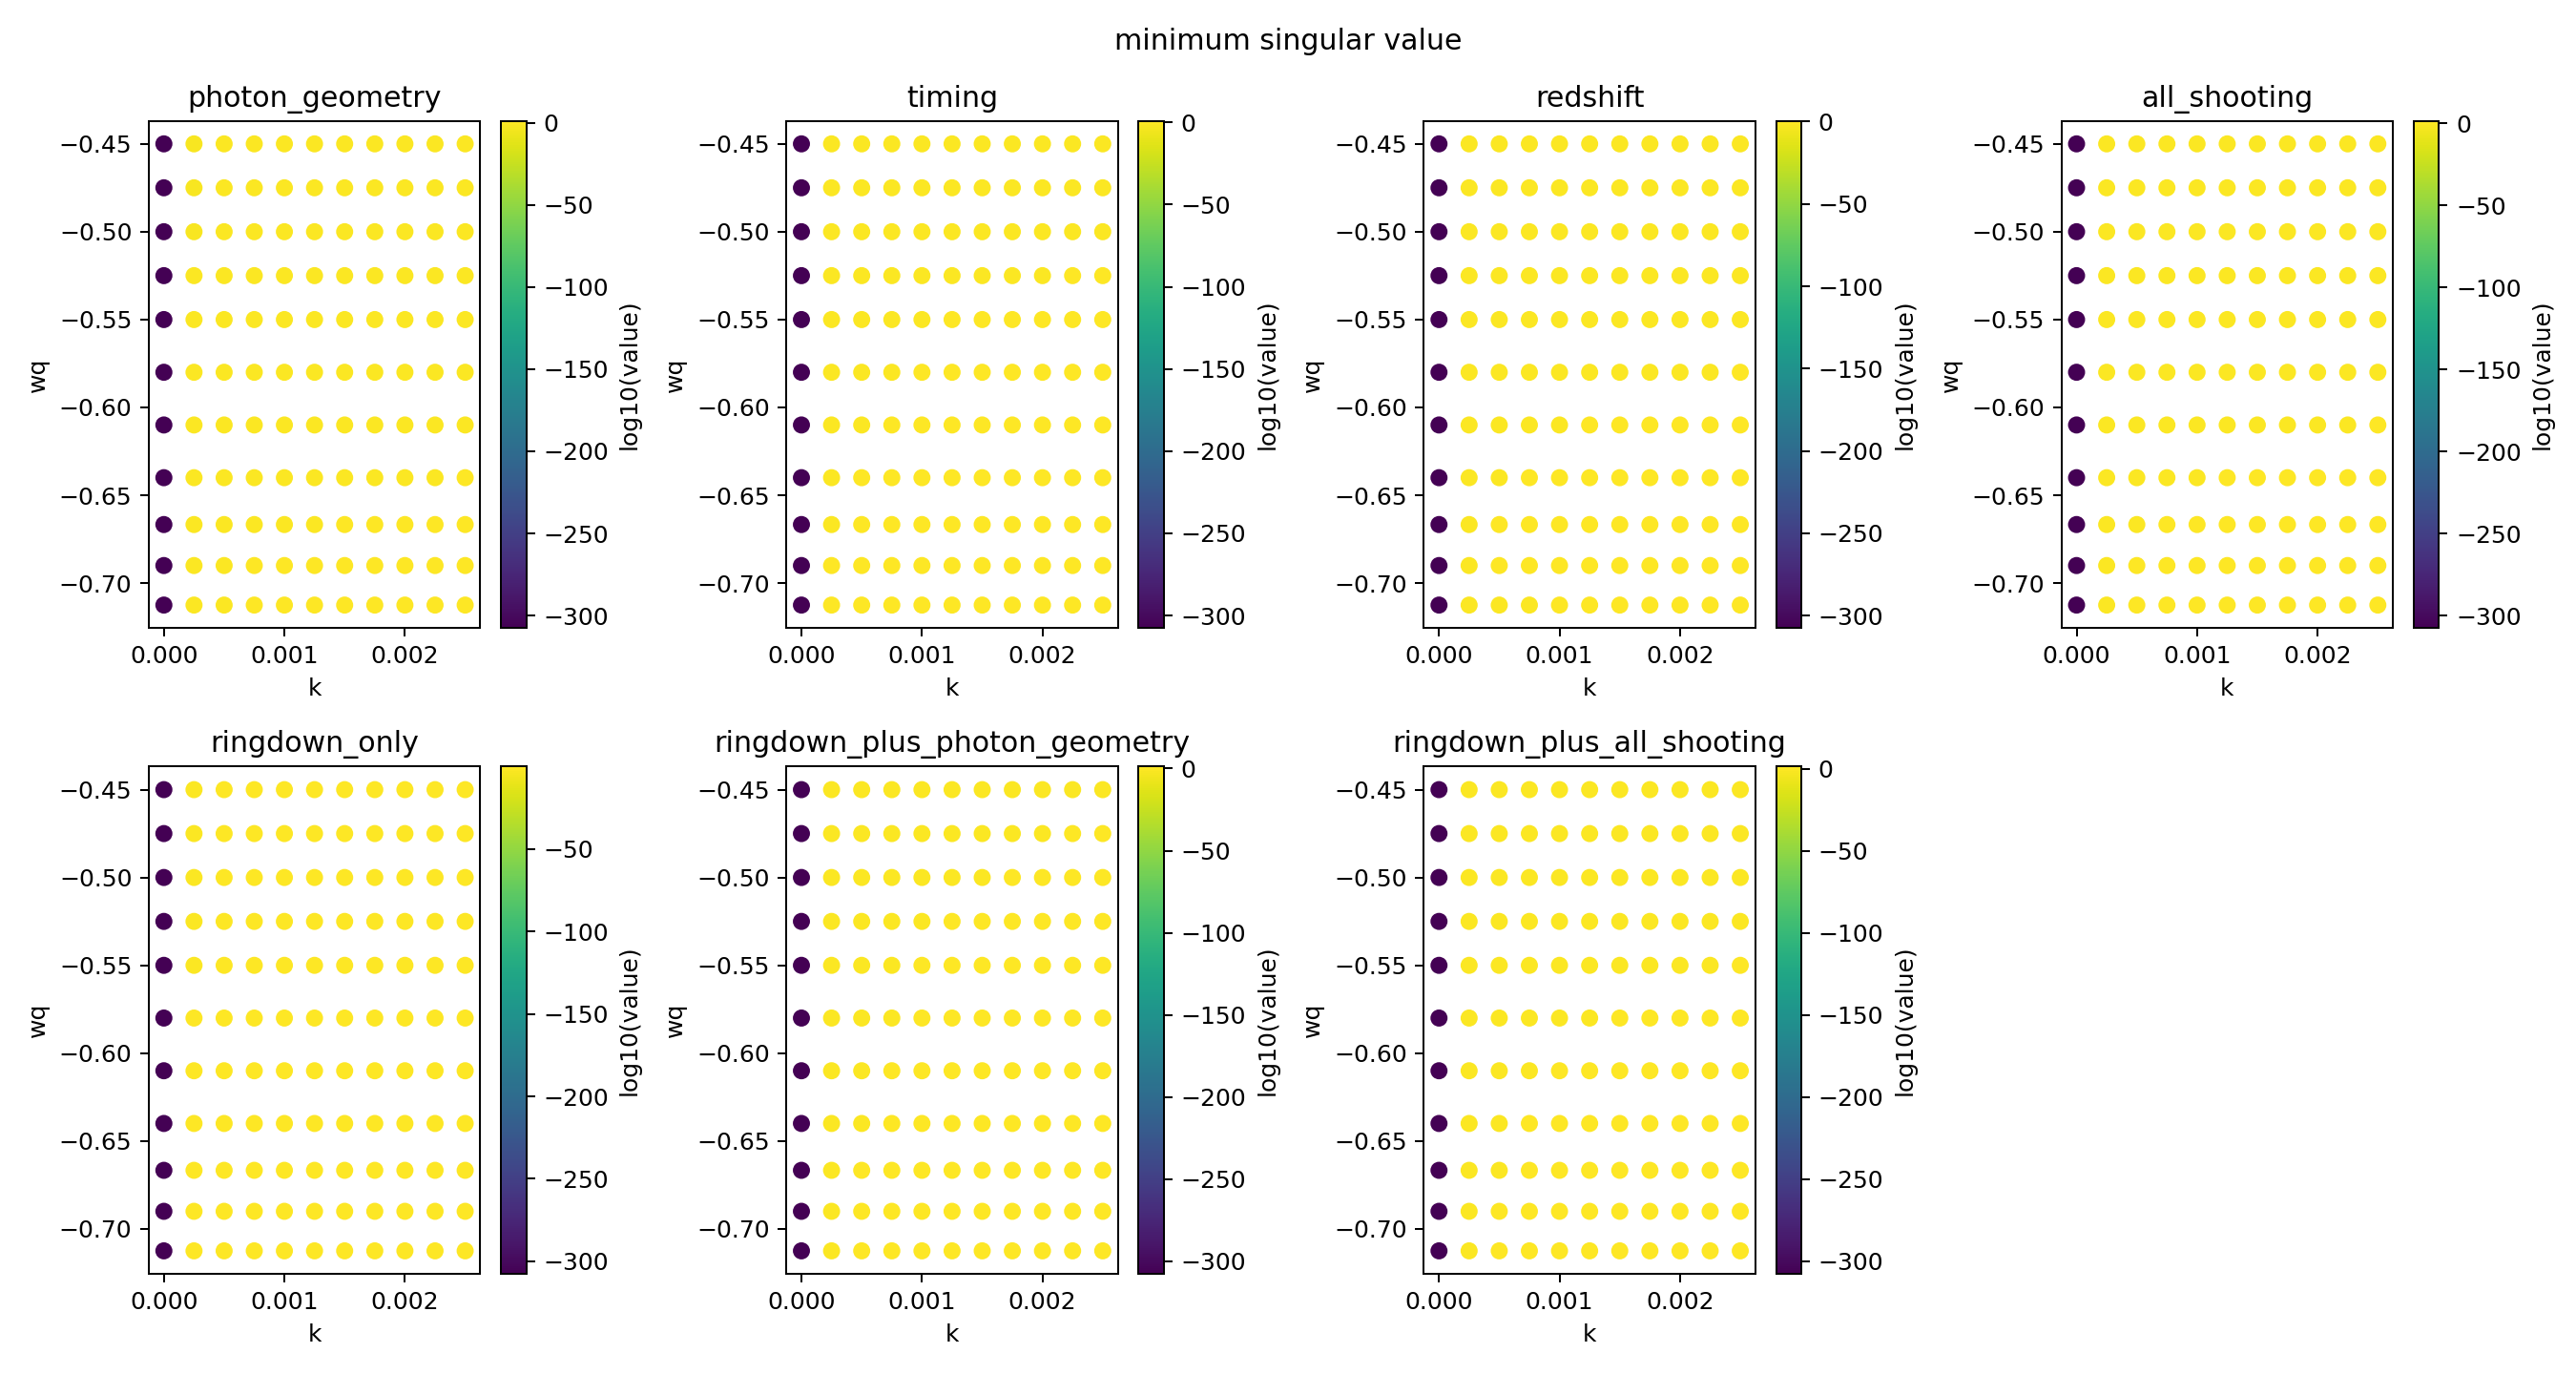
\includegraphics[width=0.92\textwidth]{physical_grid_minimum_singular_value.png}
\caption{Minimum-singular-value maps for the predeclared physical observable
sets on the accepted Kiselev science grid.}
\label{fig:physical-grid-sigma}
\end{figure*}

\begin{figure}[t]
\centering
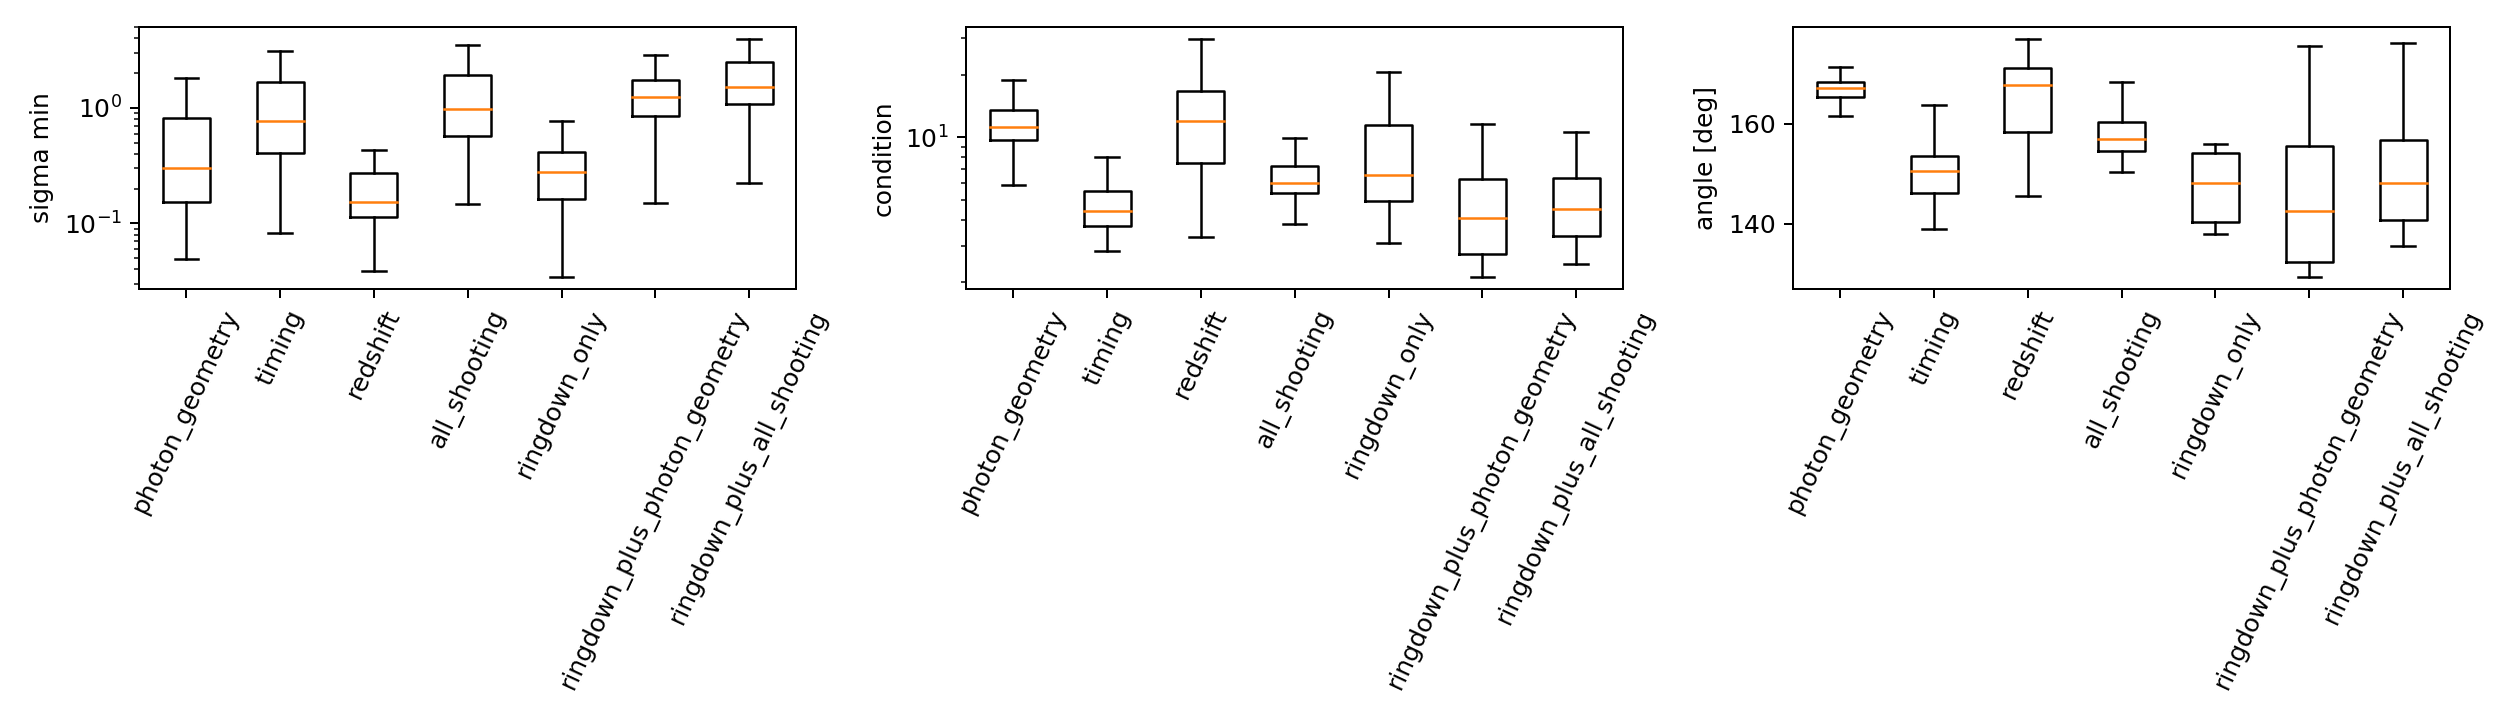
\includegraphics[width=\columnwidth]{physical_observable_complementarity.png}
\caption{Grid-wide comparison of physical observable sets.}
\label{fig:physical-complementarity}
\end{figure}

\begin{figure}[t]
\centering
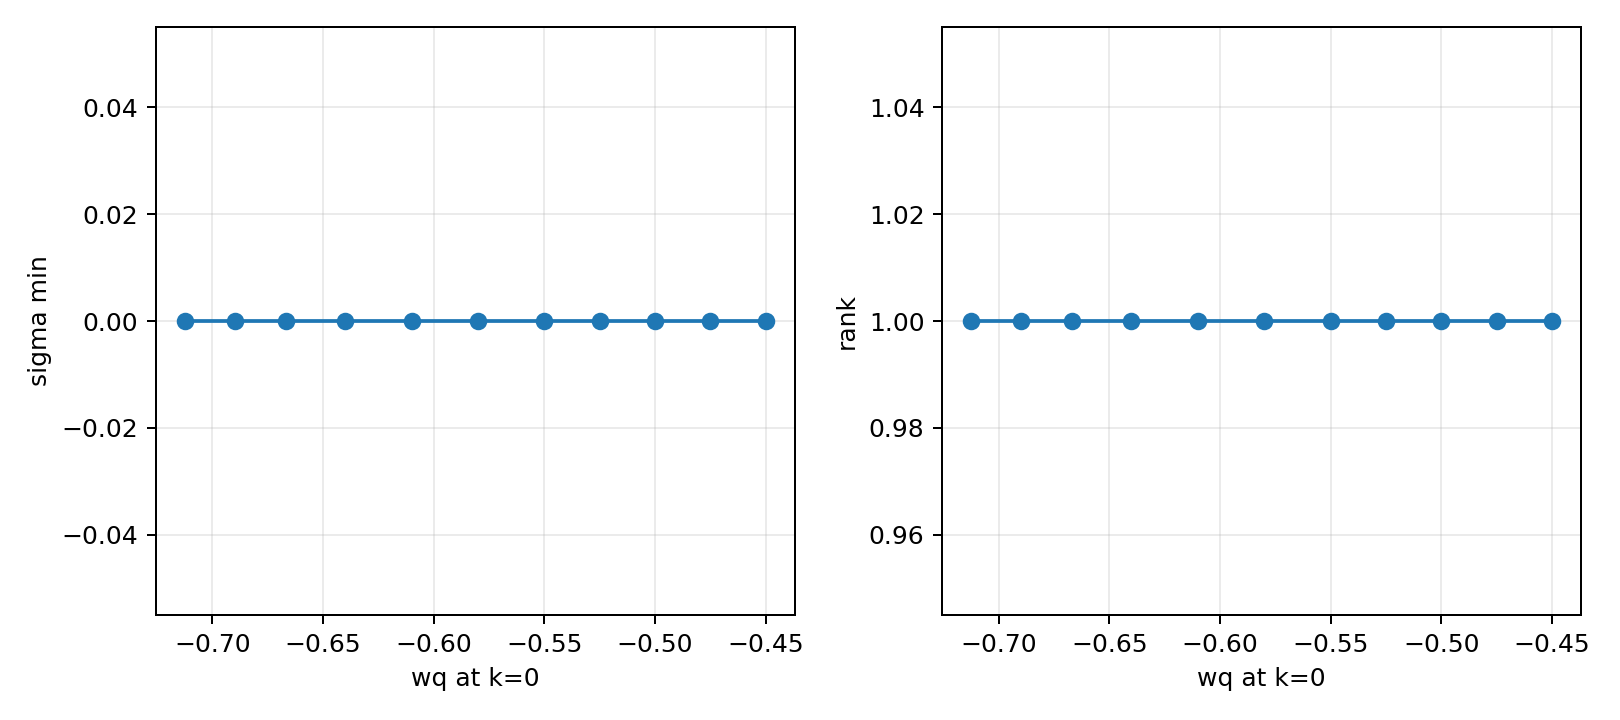
\includegraphics[width=\columnwidth]{physical_k_zero_rank_loss.png}
\caption{Exact $k=0$ rank loss: $\wq$ disappears from every physical
observable.}
\label{fig:physical-kzero}
\end{figure}

\section{Limitations and Future Work}
\textbf{Synthetic waveform scope.} The inputs are generated by
Eq.~\eqref{eq:ringdown}, not measured strain. Detector response, colored noise,
calibration error, mode mixing, and ringdown start-time uncertainty are absent,
so the noise experiment is a robustness test rather than an observational
sensitivity forecast. The mode-averaged morphology is an equal-weight feature
construction rather than an astrophysical multimode waveform with physically
inferred amplitudes and phases.

\textbf{Leading-eikonal/QNM scope.} The geodesic--QNM correspondence is a
leading-order approximation \cite{cardoso2009geodesic}. Dedicated perturbative
spectra are needed to determine whether the same observability structure
survives finite-$\ell$ corrections and waveform modeling error.

\textbf{Proxy and physical-observable scope.} The original workshop
impact-parameter, screen-coordinate, delay, and redshift features remain
synthetic proxies. They are preserved as a historical benchmark and must not be
confused with the later Hamiltonian shooting outputs. Physical shooting is now
implemented and numerically validated, but only for the direct branch, a point
emitter and point observer, a static observer, compact dimensionless geometry,
and without secondary images, radiative transfer, or a finite detector.

\textbf{Validation and extrapolation scope.} Grouped CV removes mode-level
leakage but primarily measures interpolation across the sampled family. The
physical feature grid is modest, and its final random, blocked-region, and
directional-extrapolation inverse-model results are not claimed in this
workshop update. Calibrated uncertainty, feature-noise robustness, and
simulator-mismatch studies remain necessary.

The next ray-propagation step is secondary branches, radiative transfer, and a
finite observing model. The next waveform step is validation against dedicated
Kiselev perturbative calculations, including multiple modes and finite-$\ell$
corrections. The ringdown model remains leading-eikonal, and there is no
strain-level likelihood. Only after the physical-grid inverse validation and
these modeling checks should the framework be connected to public-event
posteriors or a non-GR likelihood.

\section{Conclusion}
We presented a leakage-aware scientific-ML study of Kiselev waveform-to-hair
inference. Grouping by physical parameters and fitting PCA only on training
folds provide a credible interpolation test. Synthetic waveform morphology
recovers $(k,\wq)$ well inside the assumed simulator, while synthetic
geodesic-proxy augmentation further improves regression. More importantly, an
observability classifier learns a Fisher/Jacobian phase boundary with macro F1
0.9928, linking machine-learning errors to the local geometry of the inverse
problem. The independently evaluated $k=0$ limit establishes structural
non-identifiability, while the sampled small-nonzero-$|k|$ region reveals
full-rank but practically weak identifiability. The validated physical grid
sharpens the interpretation: large timing or redshift signals may remain poorly
identifiable when parameter responses are nearly collinear, whereas physically
complementary ringdown and photon-geometry observables improve conditioning.
Final empirical generalization on the physical feature table is deliberately
left pending. The broader AI-for-science principle is that inverse models
should learn when parameters are observable, not merely fit them.

\bibliographystyle{IEEEtran}
\bibliography{references}

\end{document}
